\documentclass[a4paper]{article}

%% Language and font encodings
\usepackage[english]{babel}
\usepackage[utf8x]{inputenc}
\usepackage[T1]{fontenc}
\usepackage{indentfirst}
\usepackage{xcolor}
\usepackage{listings}
%\usepackage{minted}


\lstdefinelanguage{json}{
  string=[s]{"}{"},
  stringstyle=\color{blue},
  comment=[l]{:},
  commentstyle=\color{black},
}


%% Sets page size and margins
\usepackage[a4paper,top=2.5cm,bottom=2.5cm,left=1.8cm,right=1.8cm]{geometry}

%% Useful packages
\usepackage{amsmath}
\usepackage{graphicx}
\usepackage[colorinlistoftodos]{todonotes}
\usepackage[colorlinks=true, allcolors=blue]{hyperref}
\usepackage{fancyhdr}
\usepackage{multirow}
\usepackage{pdflscape}
\usepackage{xcoffins}

\NewCoffin\tablecoffin
\NewDocumentCommand\Vcentre{m}
{%
  \SetHorizontalCoffin\tablecoffin{#1}%
  \TypesetCoffin\tablecoffin[l,vc]%
}

\begin{document}
%\setlength{\textwidth}{18cm}
%\setlength{\textheight}{24cm}

\title{\Huge\textbf{Cyboard}\linebreak\linebreak
  \Large\textbf{360º Company Dashboard}\linebreak\linebreak
  \large\textbf{Project Specification}\linebreak
  \linebreak\linebreak
  
\includegraphics[scale=0.1]{imgs/feup_logo.png}\linebreak\linebreak
  \linebreak\linebreak
  \Large{Master in Informatics and Computing Engineering} \linebreak\linebreak
  \Large{Information Systems}\linebreak
}

\author{\textbf{Turma 2 - Grupo A:}\\
  Ângela Filipa Pereira Cardoso, 200204375 - angela.cardoso@fe.up.pt \\
  Artur Sousa Ferreira, 201204899 - ei12168@fe.up.pt\\
  Maria Teresa dos Santos Carneiro Chaves, 201306842 - up201306842@fe.up.pt \\
  Nuno Miguel Rainho Valente, 200204376 - up200204376@fe.up.pt \\\vspace{1cm}
  \linebreak\linebreak\linebreak\linebreak\\
  Faculty of Engineering of the University of Porto \\ Rua Roberto Frias, s\/n, 4200-465 Porto, Portugal 
  \linebreak\linebreak\linebreak
  \linebreak\linebreak\vspace{1cm}
}

\maketitle
\thispagestyle{empty}

\newpage

%%%%%%%%%%%%%%%%%%%%
% PROJECT OVERVIEW %
%%%%%%%%%%%%%%%%%%%%

\section{Project Overview}

Cyboard is a fictional hardware company, which will be used to illustrate the management information needs that can be satisfied through a company dashboard.

The 360º Company Dashboard is a web application for information management, which will be developed within the curricular unit of Information Systems, a part of the Masters degree in Informatics and Computing Engineering.

This application will have as main objective to allow the Cyboard company managers access to information about the state of the company. This information will be submitted to a prior analysis, which allows the computation and visualization of Key Performance Indicators (KPIs), as well as charts with the financial, sales, purchases and stock data. For better understanding of this information, it will also be possible to verify the original documents from which it was generated. In short, the user will have a fast and simplified view of a set of complex data about the current company status.

We intend to develop this web application using an appropriate template, which we then be edited for our purpose. The frontend technology will be Angular 4 and the backend will use Node.js.

%%%%%%%%%%%%%%%%%%%
% FUNCTIONALITIES %
%%%%%%%%%%%%%%%%%%%

\section{Functionalities}

This application has a set of pages in which the user can navigate in order to achieve their objective. Figure \ref{fig:sitemap} has the sitemap, that is, it shows the application flow. Each of these pages has a set of functionalities with a main purpose. From Table \ref{table:all_funcs} to Table \ref{table:stock_funcs} we present each group of functionalities, organized by core view.

\begin{figure}[!ht]
  \begin{center}
    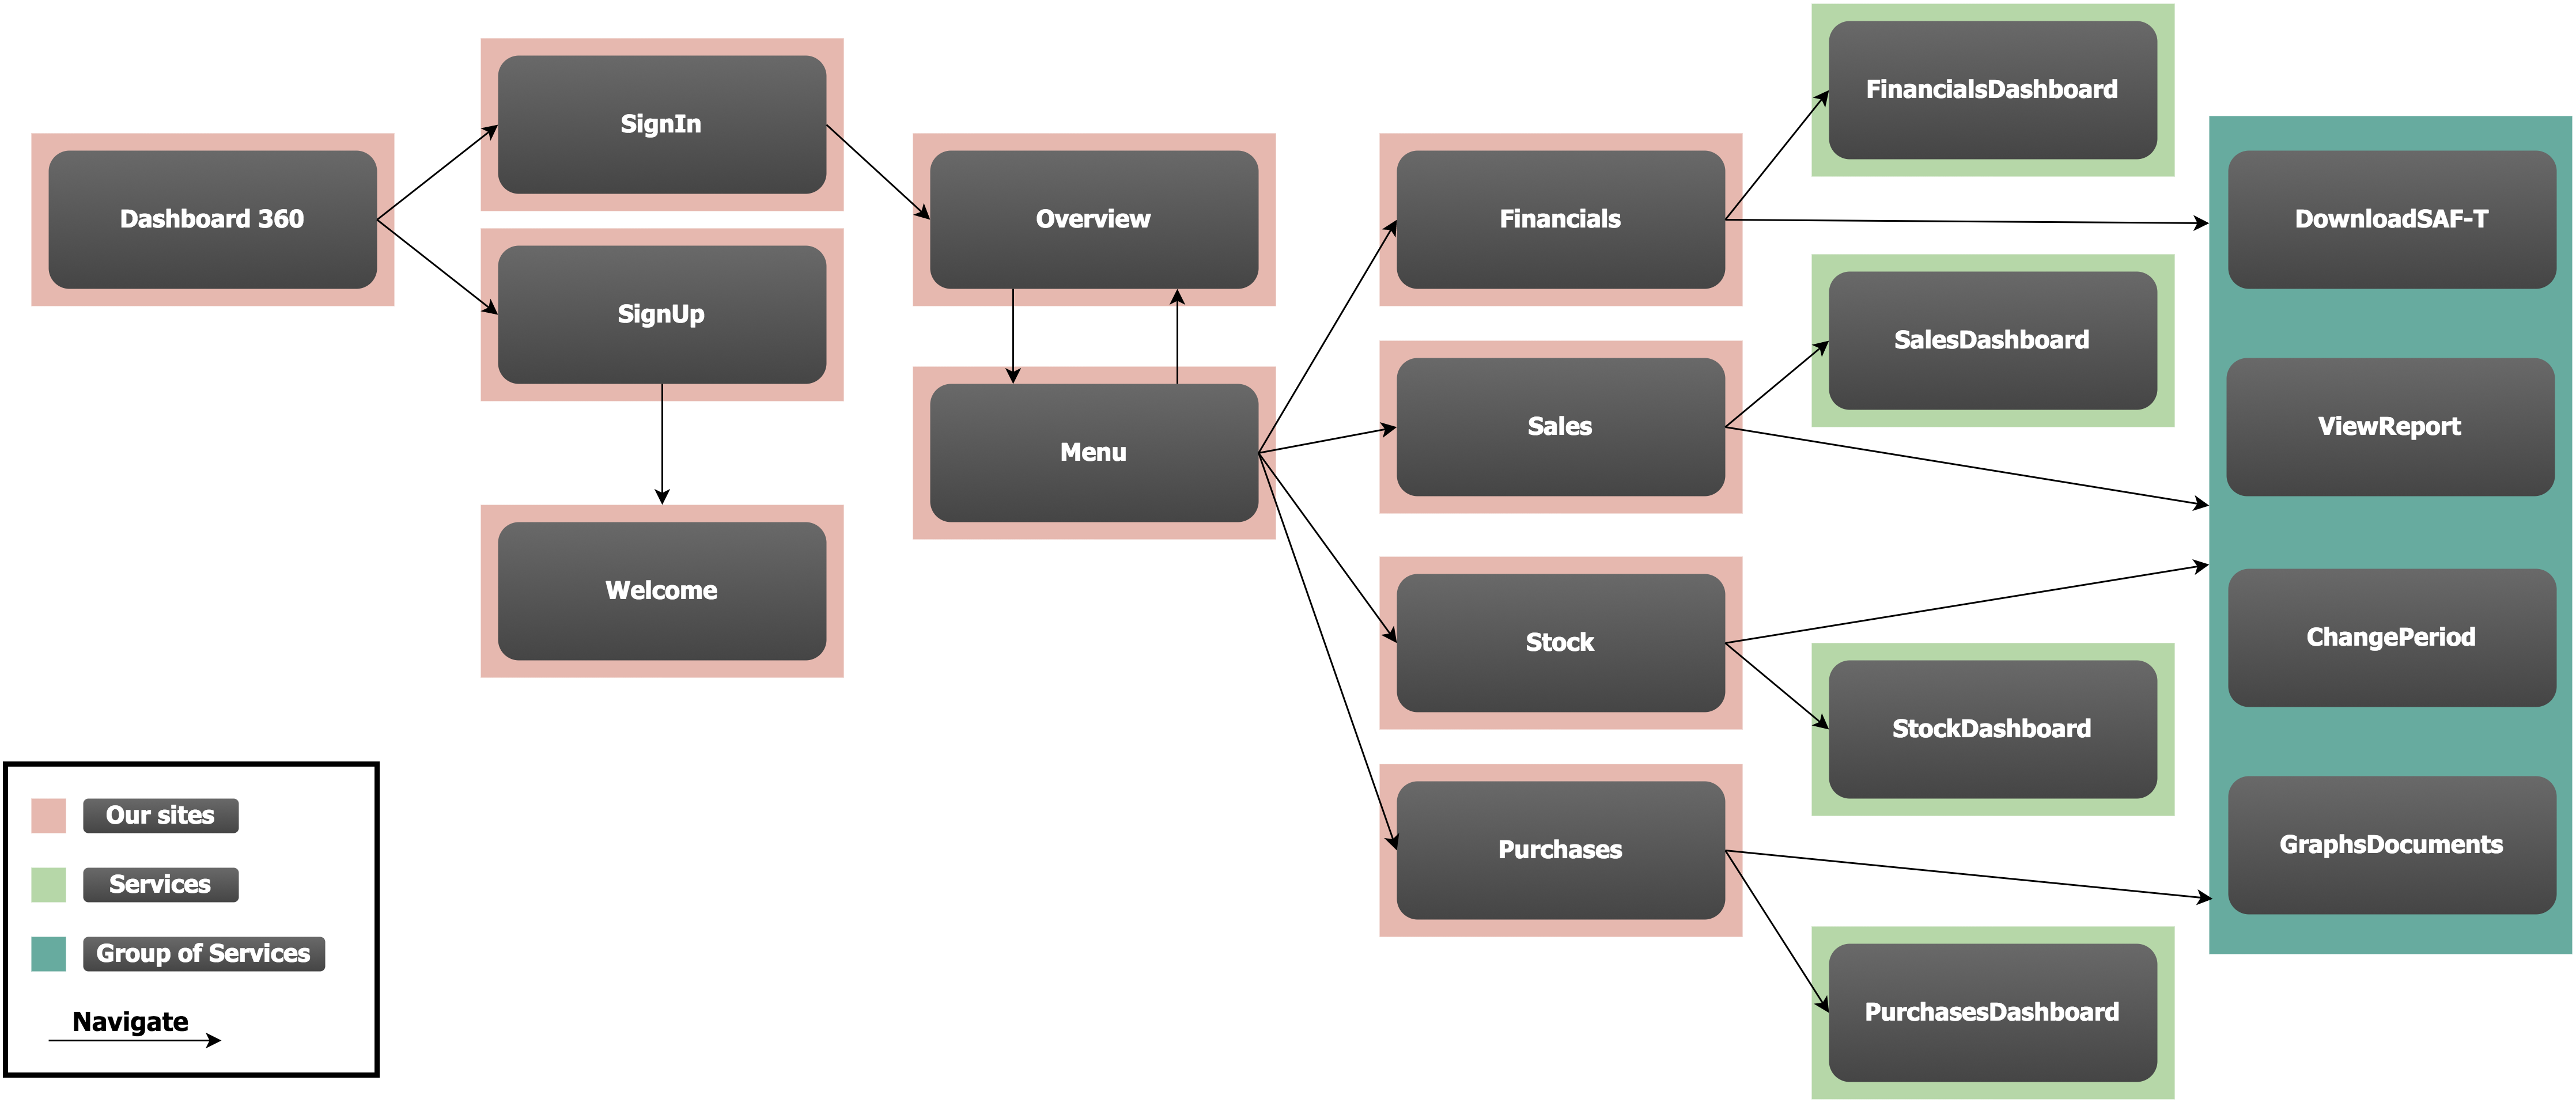
\includegraphics[width=0.9\textwidth]{imgs/sitemap.png}
    \caption{360º Company Dashboard Sitemap}
    \label{fig:sitemap}
  \end{center}
\end{figure}

% ------------------------------------------------------------

\begin{table}[!ht]
  \centering
  
  \begin{tabular}{lll}
    \textbf{CoreView} & \textbf{Functionality} & \textbf{Description} \\ \hline
                      &                        &                      \\
    \multirow{5}{*}{All} & Report           & Allows a user to view the report of the selected period \\ \cline{2-3} 
                         & Change Period    & Allows a user to change the period of the report \\ \cline{2-3} 
                         & Download SAF-T   & Allows a user to download SAF-T as csv file \\ \cline{2-3} 
                         & Menu             & Allows a user to browse through all the application pages \\ \cline{2-3} 
                         & Chart Document   & \begin{tabular}[c]{@{}l@{}}
                                                Allows a user to view the documents used to produce the\\
                                                charts presented
                                              \end{tabular}
  \end{tabular}

  \caption{Functionalities present on all the core views}
  \label{table:all_funcs}

\end{table}

\vspace{20cm}

% ------------------------------------------------------------

\begin{table}[!ht]
  \centering

  \begin{tabular}{lll}
    \textbf{CoreView}        & \textbf{Functionality}       & \textbf{Description} \\ \hline
                               &                              &            \\
    \multirow{11}{*}{Overview} & [KPI] Total Revenue & Allows a user to check the revenue of the company \\ \cline{2-3}
                & [KPI] Total Profit       & Allows a user to check the profit of the company \\ \cline{2-3} 
                & [KPI] Financial Autonomy & \begin{tabular}[c]{@{}l@{}}
                                                Allows a user to check the percentage of the company's\\
                                                financial autonomy
                                             \end{tabular} \\ \cline{2-3} 
                & [KPI] Liquidity          & Allows a user to check the company's liquidity \\ \cline{2-3} 
                & [KPI] Number of Clients  & Allows a user to check the company's number of clients \\ \cline{2-3} 
                & [KPI] Number of Sales    & Allows a user to check the company's number of sales \\ \cline{2-3} 
                & [KPI] ROE                & Allows a user to check the company's Return On Equity \\ \cline{2-3} 
                & [KPI] ROA                & Allows a user to check the company's Return on Assets \\ \cline{2-3} 
                & Top Clients              & \begin{tabular}[c]{@{}l@{}}
                                               Allows a user to analyze a chart with the company's top\\
                                               clients
                                             \end{tabular} \\ \cline{2-3} 
                & Total Costs              & Allows a user to analyze a chart with the company's costs \\ \cline{2-3} 
                & Top Sales                & Allows a user to analyze a chart with the company's sales
    \end{tabular}

  \caption{Functionalities present on the Overview core view}
  \label{table:overview_funcs}

\end{table}

% ------------------------------------------------------------

\begin{table}[!ht]
  \centering

  \begin{tabular}{lll}
    \textbf{CoreView}        & \textbf{Functionality} & \textbf{Description} \\ \hline
                             &                        &   \\
    \multirow{4}{*}{Financial} & Earnings vs Expenses & \begin{tabular}[c]{@{}l@{}}
                                                          Allows a user to analyze a chart with the company's\\
                                                          earnings and expenses
                                                        \end{tabular} \\ \cline{2-3} 
                               & \begin{tabular}[c]{@{}l@{}}
                                   Accounts Receivable\\
                                   vs Payable
                                 \end{tabular}        & \begin{tabular}[c]{@{}l@{}}
                                                          Allows a user to analyze a chart with the accounts\\
                                                          receivable and with the accounts payable
                                                        \end{tabular} \\ \cline{2-3} 
                               & \begin{tabular}[c]{@{}l@{}}
                                   Distribution of Earnings\\
                                   and Expenses
                                 \end{tabular}        & \begin{tabular}[c]{@{}l@{}}
                                                          Allows a user to analyze a chart with the distribution of \\
                                                          the company's earnings and expenses
                                                        \end{tabular} \\ \cline{2-3} 
                               & Balance Sheet        & \begin{tabular}[c]{@{}l@{}}
                                                          Allows a user to analyze a table with company's financial\\
                                                          balance
                                                        \end{tabular} \\ \cline{2-3}
  \end{tabular}

  \caption{Functionalities present on the Financial core view}
  \label{table:financial_funcs}

\end{table}

% ------------------------------------------------------------

\begin{table}[!ht]
  \centering

  \begin{tabular}{lll}
    \textbf{CoreView}      & \textbf{Functionality}                  & \textbf{Description} \\ \hline
                           &                                        &              \\
    \multirow{9}{*}{Sales} & [KPI] Total Sales Revenue          & Allows a user to check the sales revenue including AR  \\ \cline{2-3} 
                           & \begin{tabular}[c]{@{}l@{}}[KPI]
                              Total Accounts\\
                                Receivable
                             \end{tabular}              & Allows a user to check the total accounts receivable \\ \cline{2-3} 
                           & [KPI] Total Orders Amount      & Allows a user to check the total orders amount \\ \cline{2-3} 
                           & [KPI] Number of Clients      & Allows a user to check the company's number of clients \\ \cline{2-3} 
                           & [KPI] Number of Sales        & Allows a user to check the number of sales \\ \cline{2-3} 
                           & [KPI] Number of Orders       & Allows a user to check the number of orders \\ \cline{2-3} 
                           & Top Products Sold            & Allows a user to analyze a chart with the top products sold \\ \cline{2-3} 
                           & Cost of Products Sold          & \begin{tabular}[c]{@{}l@{}}
                                                    Allows a user to analyze a chart with the cost of products\\
                                                                            sold
                                                                      \end{tabular} \\ \cline{2-3} 
                           & Online vs In-Store sales         & \begin{tabular}[c]{@{}l@{}}
                                                    Allows a user to analyze a chart with the amount of online\\
                                                                            vs in-store sales
                                                                      \end{tabular}
  \end{tabular}

  \caption{Functionalities present on the Sales core view}
  \label{table:sales_funcs}
\end{table}

\vspace{20cm}

% ------------------------------------------------------------

\begin{table}[!ht]
\centering

  \begin{tabular}{lll}
    \textbf{CoreView}          & \textbf{Functionality}         & \textbf{Description} \\ \hline
                               &                                        &              \\
    \multirow{9}{*}{Purchases} & [KPI] Total Purchases Cost         & \begin{tabular}[c]{@{}l@{}}
                                          Allows a user to check the total purchases cost including\\ 
                                                                                AP
                                                                          \end{tabular} \\ \cline{2-3} 
                               & \begin{tabular}[c]{@{}l@{}}[KPI]
                                    Total Accounts\\
                                        Payable\end{tabular}      & Allows a user to check the total accounts payable \\ \cline{2-3} 
                               & [KPI] Total Orders Amount      & Allows a user to check the total orders amount \\ \cline{2-3} 
                               & [KPI] Number of Suppliers      & Allows a user to check the number of suppliers \\ \cline{2-3} 
                               & [KPI] Number of Purchases      & Allows a user to check the number of purchases \\ \cline{2-3} 
                               & [KPI] Number of Orders       & Allows a user to check the number of orders \\ \cline{2-3} 
                               & Top Products Purchased         & \begin{tabular}[c]{@{}l@{}}
                                                        Allows a user to analyze a chart with the top products\\
                                                                                purchased
                                                                          \end{tabular} \\ \cline{2-3} 
                               & Purchases per Sector         & \begin{tabular}[c]{@{}l@{}}
                                                        Allows a user to analyze a chart with the purchases per\\
                                                                                sector
                                                                          \end{tabular} \\ \cline{2-3} 
                               & \begin{tabular}[c]{@{}l@{}}
                                    Amount of Imported\\
                                        vs National
                                 \end{tabular}                & \begin{tabular}[c]{@{}l@{}}
                                                        Allows a user to analyze a chart with the amount of\\
                                                                                imported vs national
                                                                          \end{tabular}
  \end{tabular}

  \caption{Functionalities present on the Purchases core view}
  \label{table:purchases_funcs}
\end{table}

% ------------------------------------------------------------

\begin{table}[!ht]
  \centering

  \begin{tabular}{lll}
    \textbf{CoreView}      & \textbf{Functionality}         & \textbf{Description} \\ \hline
                           &                    &              \\
    \multirow{7}{*}{Stock} & Search Product Stock         & \begin{tabular}[c]{@{}l@{}}
                                        Allows a user to search existent stock product by location,\\
                                                                            date and reference
                                                                      \end{tabular} \\ \cline{2-3}
                           & Stock Level and Value                  & \begin{tabular}[c]{@{}l@{}}
                                                  Allows a user to view the changes in stock level and value\\
                                                                            over time
                                                                      \end{tabular} \\ \cline{2-3} 
                           & \begin{tabular}[c]{@{}l@{}}[KPI]
                                Stock Level\\
                                    by Location
                             \end{tabular}              & Allows a user to check the stock level in each location                                                                         \\ \cline{2-3} 
                           & \begin{tabular}[c]{@{}l@{}}[KPI]
                                Stock Value\\
                                    by Location
                             \end{tabular}              & Allows a user to check the stock value in each location \\ \cline{2-3} 
                           & Top Used Suppliers           & Allows a user to analyze a chart with the top used suppliers \\ \cline{2-3} 
                           & Top Products Sold            & Allows a user to analyze a chart with the top products sold \\ \cline{2-3} 
                           & \begin{tabular}[c]{@{}l@{}}
                              Locations With More\\
                                Stock Level
                             \end{tabular}              & \begin{tabular}[c]{@{}l@{}}
                                                    Allows a user to analyze a chart with the number of X locations\\
                                                                            with more stock level
                                                                      \end{tabular} \\ \cline{2-3} 
  \end{tabular}

  \caption{Functionalities present on the Stock core view}
  \label{table:stock_funcs}
\end{table}


%%%%%%%%%%%%%%%%%%%%%%%%%%%%
% INFORMATION ARCHITECTURE %
%%%%%%%%%%%%%%%%%%%%%%%%%%%%

\section{Information Architecture}

In this section, we identify the core views of our application, that is, we describe the main pages (since this will be a website) of our product. This way, it becomes clear what are the main things a user can do and see within the application. 

For each core view, we also present the main user goals, the ways to access that view (inwards) and what is possible to do once in there (outwards).

We decided to have a main transversal view - Overview - that contains the key information for the company general manager. From there it is possible to  access all the other core views. These other views where identified according to the projected management needs of an hardware company, but they are pretty much the same for most companies: financial, sales, purchases and stock.


%%%%%%%%%%%%
% OVERVIEW %
%%%%%%%%%%%%
\begin{landscape}
\thispagestyle{empty}

\subsection{Overview}

\begin{tabular}{ccc}

  \Vcentre{}
    & \Vcentre{
    \begin{tabular} {l}
      \textbf{USER BUSINESS GOALS}\\ \hline
      - Company overview \\
      - To be used as a management tool and quick view of the company status
    \end{tabular}
  }
    & \Vcentre{} \\
    
    \Vcentre{}
    & \Vcentre{}
    & \Vcentre{} \\
  
    \Vcentre{
    \begin{tabular} {l}
      \textbf{INWARDS} \\ \hline
      - Sign In \\
      - Menu
    \end{tabular}
  }
    & \Vcentre{
    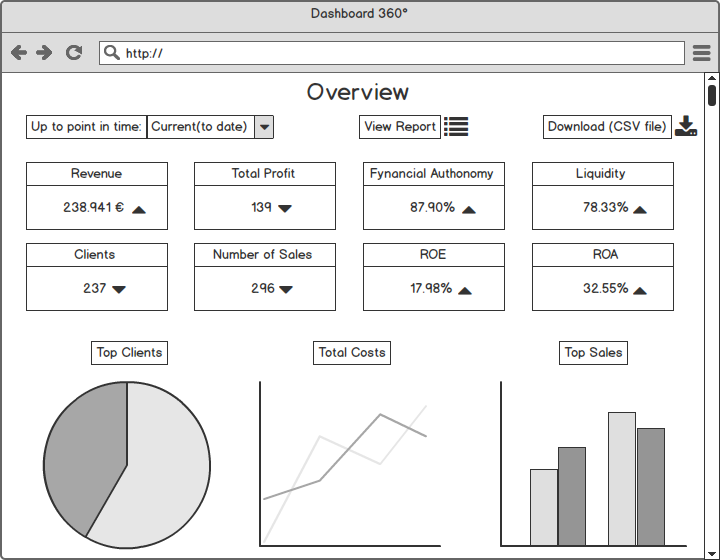
\includegraphics[scale=0.6]{imgs/Overview.png}
    }
    & \Vcentre{
    \begin{tabular} {l}
      \textbf{OUTWARDS} \\ \hline
      - Menu \\
            - Download SAF-T as csv file \\
            - View the report \\
            - Change the period \\
              of the report \\
            - View documents about \\
              the charts produced
    \end{tabular}
  } \\
      
  \Vcentre{}
    & \Vcentre{}
    & \Vcentre{} \\
      
    \Vcentre{}
    & \Vcentre{
    \begin{tabular} {l}
      \textbf{ELEMENTS OF THE CORE} \\ \hline
      - KPI\_01 | Total Revenue \hspace{1.1cm}
            - KPI\_02 | Total Profit \hspace{1cm}
            - KPI\_03 | Company's Financial Autonomy \\
      - KPI\_04 | Company's liquidity \hspace{0.2cm}
            - KPI\_05 | Number of Clients \hspace{0cm}
      - KPI\_06 | Number of Sales \\
            - KPI\_07 | Return On Equity \hspace{0.5cm}
            - KPI\_08 | Return on Assets \hspace{0.2cm}
            - PIE\_01 | Top Clients \\
            - LINE\_01 | Total Costs \hspace{1.3cm}
      - BAR\_01 | Top Sales
    \end{tabular}
  }
    & \Vcentre{} \\
    
\end{tabular}

\vfill
\raisebox{0cm}{\makebox[\linewidth]{\thepage}}
\end{landscape}
\newpage


%%%%%%%%%%%%%
% FINANCIAL %
%%%%%%%%%%%%%
\begin{landscape}
\thispagestyle{empty}

\subsection{Financial View}

\begin{tabular}{ccc}

  \Vcentre{}
    & \Vcentre{
    \begin{tabular} {l}
      \textbf{USER BUSINESS GOALS}\\ \hline
      - Monitoring the financial area and accounting \\
            - Inform the user about the data entered in the accounting
    \end{tabular}
  }
    & \Vcentre{} \\
    
    \Vcentre{}
    & \Vcentre{}
    & \Vcentre{} \\
  
    \Vcentre{
    \begin{tabular} {l}
      \textbf{INWARDS} \\ \hline
      - Overview \\
      - Menu
    \end{tabular}
  }
    & \Vcentre{
    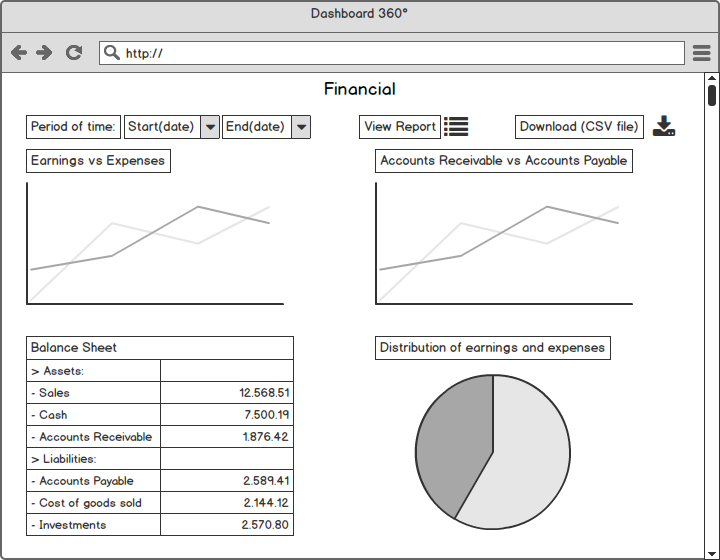
\includegraphics[scale=0.6]{imgs/Financials.png}
    }
    & \Vcentre{
    \begin{tabular} {l}
      \textbf{OUTWARDS} \\ \hline
      - Menu \\
            - Download SAF-T as csv file \\
      - View the report \\
      - Change the period \\
        of the report \\
      - View documents about \\
        the charts produced
    \end{tabular}
  } \\
      
  \Vcentre{}
    & \Vcentre{}
    & \Vcentre{} \\
      
    \Vcentre{}
    & \Vcentre{
    \begin{tabular} {l}
      \textbf{ELEMENTS OF THE CORE} \\ \hline
        - LINE\_02 | Earnings vs Expenses \hspace{2cm}
        - LINE\_03 | Accounts Receivable vs Payable \\
        - KPI\_09 | Total Assets Amount \hspace{2.25cm}
        - KPI\_10 | Sales Amount \\
        - KPI\_11 | Cash Amount \hspace{3.4cm} 
        - KPI\_12 | Accounts Receivable Amount \\
        - KPI\_13 | Total Liabilities Amount \hspace{1.7cm}
        - KPI\_14 | Accounts Payable Amount \\
        - KPI\_15 | Cost of Goods Sold Amount \hspace{1.2cm}
        - KPI\_16 | Investments Amount \\
        - PIE\_02 | Distribution of Earnings and Expenses 
    \end{tabular}
  }
  & \Vcentre{} \\
    
\end{tabular}

%\vfill
%\raisebox{0cm}{\makebox[\linewidth]{\thepage}}
\end{landscape}
\newpage


%%%%%%%%%
% SALES %
%%%%%%%%%
\begin{landscape}
\thispagestyle{empty}

\subsection{Sales View}

\begin{tabular}{ccc}

  \Vcentre{}
    & \Vcentre{
    \begin{tabular} {l}
      \textbf{USER BUSINESS GOALS}\\ \hline
      - Company sales view \\
      - View to be used as a sales management tool
    \end{tabular}
  }
    & \Vcentre{} \\
    
    \Vcentre{}
    & \Vcentre{}
    & \Vcentre{} \\
  
    \Vcentre{
    \begin{tabular} {l}
      \textbf{INWARDS} \\ \hline
      - Overview \\
      - Menu
    \end{tabular}
  }
    & \Vcentre{
    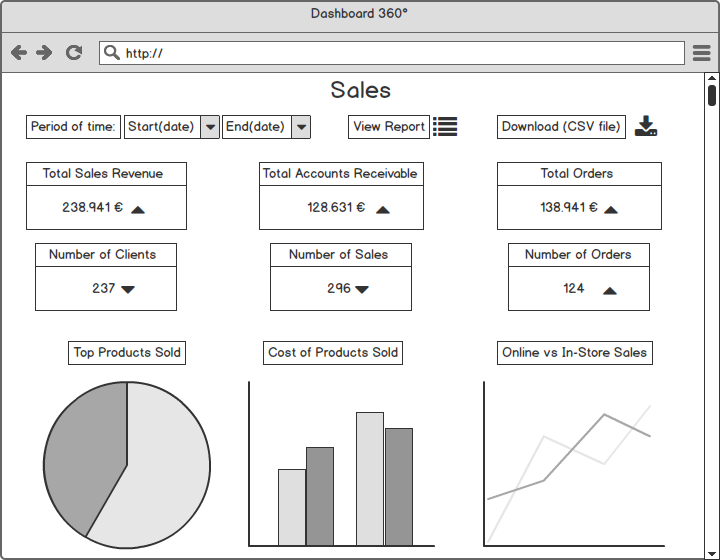
\includegraphics[scale=0.6]{imgs/Sales.png}
    }
    & \Vcentre{
    \begin{tabular} {l}
      \textbf{OUTWARDS} \\ \hline
      - Menu \\
            - Download SAF-T as csv file \\
      - View the report \\
      - Change the period \\
        of the report \\
      - View documents about \\
        the charts produced
    \end{tabular}
  } \\
      
  \Vcentre{}
    & \Vcentre{}
    & \Vcentre{} \\
      
    \Vcentre{}
    & \Vcentre{
    \begin{tabular} {l}
      \textbf{ELEMENTS OF THE CORE} \\ \hline
      - KPI\_17 | Total Sales Revenue Including AR \hspace{1.1cm}
            - KPI\_18 | Total Accounts Receivable \\
            - KPI\_19 | Total Orders Amount \hspace{3.1cm}
      - KPI\_20 | Number of Clients \\
            - KPI\_21 | Number of Sales \hspace{3.9cm}
      - KPI\_22 | Number of Orders \\
            - PIE\_03 | Top Products Sold \hspace{3.6cm}
            - BAR\_02 | Cost of Products Sold \\
      - LINE\_04 | Amount of Online vs In-Store sales
    \end{tabular}
  }
    & \Vcentre{} \\
    
\end{tabular}

\vfill
\raisebox{0cm}{\makebox[\linewidth]{\thepage}}
\end{landscape}
\newpage


%%%%%%%%%%%%%
% PURCHASES %
%%%%%%%%%%%%%
\begin{landscape}
\thispagestyle{empty}

\subsection{Purchases View}

\begin{tabular}{ccc}

  \Vcentre{}
    & \Vcentre{
    \begin{tabular} {l}
      \textbf{USER BUSINESS GOALS}\\ \hline
      - Company purchases view \\
            - View to be used as a purchases management tool
    \end{tabular}
  }
    & \Vcentre{} \\
    
    \Vcentre{}
    & \Vcentre{}
    & \Vcentre{} \\
  
    \Vcentre{
    \begin{tabular} {l}
      \textbf{INWARDS} \\ \hline
      - Overview \\
      - Menu
    \end{tabular}
  }
    & \Vcentre{
    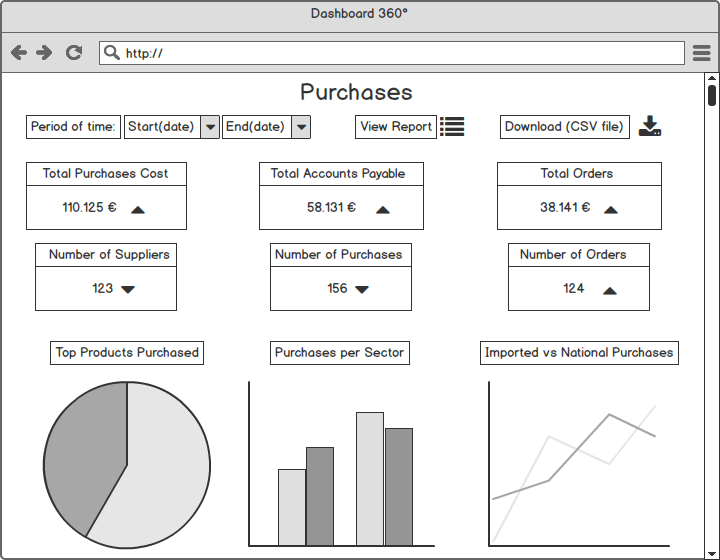
\includegraphics[scale=0.6]{imgs/Purchases.png}
    }
    & \Vcentre{
    \begin{tabular} {l}
      \textbf{OUTWARDS} \\ \hline
      - Menu \\
            - Download SAF-T as csv file \\
      - View the report \\
      - Change the period \\
        of the report \\
      - View documents about \\
        the charts produced
    \end{tabular}
  } \\
      
  \Vcentre{}
    & \Vcentre{}
    & \Vcentre{} \\
      
    \Vcentre{}
    & \Vcentre{
    \begin{tabular} {l}
      \textbf{ELEMENTS OF THE CORE} \\ \hline
      - KPI\_23 | Total Purchases Cost Including AP \hspace{1.4cm}
            - KPI\_24 | Total Accounts Payable \\
            - KPI\_25 | Total Orders Amount \hspace{3.5cm}
      - KPI\_26 | Number of Suppliers \\
            - KPI\_27 | Number of Purchases \hspace{3.6cm}
      - KPI\_28 | Number of Orders \\
            - PIE\_04| Top Products Purchased \hspace{3.1cm}
            - BAR\_03 | Purchases per Sector \\
      - LINE\_05 | Amount of Imported vs National Purchases
    \end{tabular}
  }
    & \Vcentre{} \\
    
\end{tabular}

\vfill
\raisebox{0cm}{\makebox[\linewidth]{\thepage}}
\end{landscape}
\newpage



%%%%%%%%%
% STOCK %
%%%%%%%%%
\begin{landscape}
\thispagestyle{empty}

\subsection{Stock View}

\begin{tabular}{ccc}

  \Vcentre{}
    & \Vcentre{
    \begin{tabular} {l}
      \textbf{USER BUSINESS GOALS}\\ \hline
      - Company stock view \\
            - Presentation of key stock metrics
    \end{tabular}
  }
    & \Vcentre{} \\
    
    \Vcentre{}
    & \Vcentre{}
    & \Vcentre{} \\
  
    \Vcentre{
    \begin{tabular} {l}
      \textbf{INWARDS} \\ \hline
      - Overview \\
      - Menu
    \end{tabular}
  }
    & \Vcentre{
    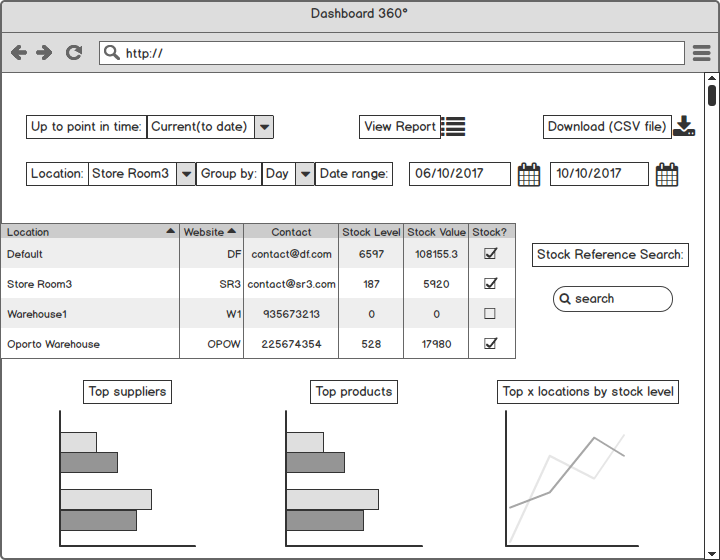
\includegraphics[scale=0.6]{imgs/Stock.png}
    }
    & \Vcentre{
    \begin{tabular} {l}
      \textbf{OUTWARDS} \\ \hline
      - Menu \\
            - Download SAF-T as csv file \\
      - View the report \\
      - Change the period \\
        of the report \\
            - View documents about \\
              the charts produced \\ 
      - Search existent stock \\
        product by location, \\
        date and reference \\ 
            - View the change in stock \\
              level and value over time
    \end{tabular}
  } \\
      
  \Vcentre{}
    & \Vcentre{}
    & \Vcentre{} \\
      
    \Vcentre{}
    & \Vcentre{
    \begin{tabular} {l}
      \textbf{ELEMENTS OF THE CORE} \\ \hline
      - KPI\_29 | Stock level in each location \\
            - KPI\_30 | Stock value in each location \\
            - BAR\_04 | Top used suppliers \\
            - BAR\_05 | Top products sold \\
      - LINE\_06 | Number of X locations with more stock level
    \end{tabular}
  }
    & \Vcentre{} \\
    
\end{tabular}

\vfill
\raisebox{0cm}{\makebox[\linewidth]{\thepage}}
\end{landscape}
\newpage

%%%%%%%%%%%%%%%%%%%%%%%%%%%%%%%%%%%
% INTEROPERABILITY WITH PRIMAVERA %
%%%%%%%%%%%%%%%%%%%%%%%%%%%%%%%%%%%
\section{Interoperability with Primavera}

In this chapter we present the implementation of the interoperability layer and
web services required for the core views defined above.


% ---------------------------------
\subsection{Financial}

\begin{itemize}
  \item \textbf{Webservice ID:} $getBalanceSheet$
  \item \textbf{Description:} returns the balance sheet within a range of dates
  \item \textbf{Related core views:} Overview, Financial View
  \item \textbf{Related KPIs:} KPI\_09, KPI\_10, KPI\_11,  KPI\_12, KPI\_13, KPI\_14, KPI\_15, KPI\_16
  \item \textbf{Route and verbs:} /api/primavera/balance GET
  \item \textbf{Input example:} $init=yyyy/mm/dd\&end=yyyy/mm/dd$
  \item \textbf{Expected output:} 

  \lstinputlisting[language=json]{src/getBalanceSheet.json}
\end{itemize}


% ---------------------------------
\subsection{Sales}

\begin{itemize}
  \item \textbf{Webservice ID:} $getSales$
  \item \textbf{Description:} returns a list of sales within a range of dates
  \item \textbf{Related core views:} Overview, Financial View, Sales View
  \item \textbf{Related KPIs:} KPI\_06, KPI\_10, KPI\_17, KPI\_21
  \item \textbf{Route and verbs:} /api/primavera/sale GET
  \item \textbf{Input example:} $init=yyyy/mm/dd\&end=yyyy/mm/dd$
  \item \textbf{Expected output:} 

  \lstinputlisting[language=json]{src/getSales.json}
\end{itemize}


% ---------------------------------
\subsection{Purchases}

\begin{itemize}
  \item \textbf{Webservice ID:} $getPurchases$
  \item \textbf{Description:} returns a list of purchases within a range of dates
  \item \textbf{Related core views:} Overview, Purchases View
  \item \textbf{Related KPIs:} KPI\_07, KPI\_08, KPI\_23, KPI\_24, KPI\_26, KPI\_27, KPI\_28
  \item \textbf{Route and verbs:} /api/primavera/purchase GET
  \item \textbf{Input example:} $init=yyyy/mm/dd\&end=yyyy/mm/dd$
  \item \textbf{Expected output:} 

  \lstinputlisting[language=json]{src/getPurchases.json}
\end{itemize}


% ---------------------------------
\subsection{Receivables}

\begin{itemize}
  \item \textbf{Webservice ID:} $getReceivables$
  \item \textbf{Description:} returns a list of receivables within a range of dates
  \item \textbf{Related core views:} Financial View, Sales View
  \item \textbf{Related KPIs:} KPI\_12, KPI\_18
  \item \textbf{Route and verbs:} /api/primavera/receivable GET
  \item \textbf{Input example:} $init=yyyy/mm/dd\&end=yyyy/mm/dd$
  \item \textbf{Expected output:} 

  \lstinputlisting[language=json]{src/getReceivables.json}
\end{itemize}


% ---------------------------------
\subsection{Payables}

\begin{itemize}
  \item \textbf{Webservice ID:} $getPayables$
  \item \textbf{Description:} returns a list of payables within a range of dates
  \item \textbf{Related core views:} Financial View, Purchases View
  \item \textbf{Related KPIs:} KPI\_14, KPI\_24
  \item \textbf{Route and verbs:} /api/primavera/payable GET
  \item \textbf{Input example:} $init=yyyy/mm/dd\&end=yyyy/mm/dd$
  \item \textbf{Expected output:} 

  \lstinputlisting[language=json]{src/getPayables.json}
\end{itemize}



%%%%%%%%%%%%%%%%%%%%
% PROJECT SCHEDULE %
%%%%%%%%%%%%%%%%%%%%
\begin{landscape}
\thispagestyle{empty}
\section{Project Execution Plan}

In Figure~\ref{fig:gantt} we present our projected time frame for developing this project.

\begin{figure}[!ht]
    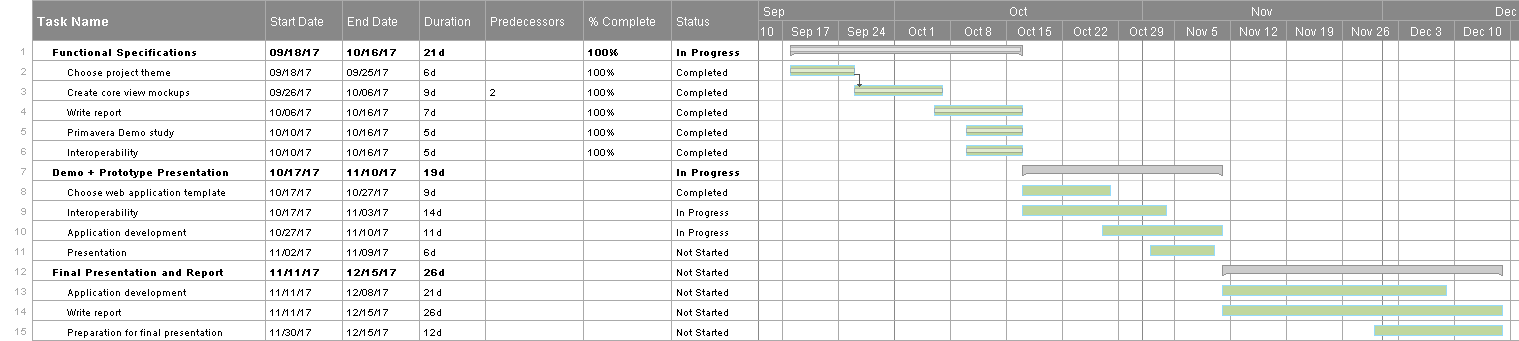
\includegraphics[width=1.4\textwidth]{imgs/gantt.png}
    \caption{Project Gantt Diagram}
    \label{fig:gantt}
\end{figure}


%%%%%%%%%%%%%%
% REFERENCES %
%%%%%%%%%%%%%%

\nocite{business_dashboard}
\nocite{kpis_def}
\nocite{business_dashboards}

\bibliographystyle{alpha}
\bibliography{sample}

\vfill
\raisebox{0cm}{\makebox[\linewidth]{\thepage}}
\end{landscape}


\end{document}